\documentclass{report}
\usepackage[T1]{fontenc}
\usepackage[utf8]{inputenc}
\usepackage{lmodern}
%\usepackage{hyperref}
\usepackage[portuges,brazilian]{babel}
\usepackage{graphicx}
\usepackage{textcomp}
\usepackage{fullpage}
\usepackage{wrapfig}
\usepackage{float}
\usepackage{listings}
\usepackage{amsmath}
\usepackage{amssymb}
\begin{document}

\newcommand{\HRule}{\rule{\linewidth}{0.5mm}}
\newcommand{\tsize}[1]{(\frac{W}{L})_{#1}}
 

%%%%%%%%%%%%%%%%%%%%%%%%%% START TITLE PAGE %%%%%%%%%%%%%%%%%%%%%%%%5
\begin{titlepage}

\begin{center}


{\LARGE UNIVERSIDADE DE SÃO PAULO\\}
{\LARGE DEPARTAMENTO DE ENGENHARIA ELÉTRICA \\}
{\LARGE ESCOLA DE ENGENHARIA DE SÃO CARLOS\\[4cm]}

\textbf{\large SEL5755 - Sistemas Fuzzy}\\[1cm]
\textbf{\large Prof Dr. Ivan Nunes da Silva}\\[2cm]


% Title
\HRule \\[0.6cm]
{ \huge EPC 2\bfseries }\\[0.6cm]

\HRule \\[2cm]

% Author

\begin{center} \large
\emph{Alunos:}\\
\end{center}

\begin{minipage}{0.4\textwidth}
\begin{flushleft} \large
Isabela R. do Prado \textsc{Rossales}\\
6445435
\end{flushleft}
\end{minipage}
\begin{minipage}{0.4\textwidth}
\begin{flushright} \large
Jonas Rossi \textsc{Dourado}\\
6445442
\end{flushright}
\end{minipage}

\vfill

% Bottom of the page
{\large São Carlos,\\ \today}

\end{center}

\end{titlepage}
%\listoffigures
%\begingroup
%\let\clearpage\relax
%\listoftables
%\endgroup
%%%%%%%%%%%%%%%%%%%%%%%%%% STOP TITLE PAGE %%%%%%%%%%%%%%%%%%%%%%%%5


\newpage

\begin{enumerate}

\item[1] Considere o conjunto \emph{fuzzy} A definido no universo de discurso $X = \{ x \in  \mathbb{R} \vert 0 \le x \le 10\}$,
o qual é representado pela seguinte função de pertinência:


\begin{equation*}
\mu_A (x) = 
\begin{cases} 
0,5x-1,5, & \text{se $3 \leq x \leq 5$}
\\
-0,5x+3,5, & \text{se $5 < x \leq 7$}
\\
0, &\text{caso contrário}
\end{cases}
\end{equation*}

\begin{enumerate}
    \item[a)] Esboce o gráfico da função de pertinência representada acima, indicando também qual é o seu tipo.

        \begin{figure}[hptb]
        \centering
        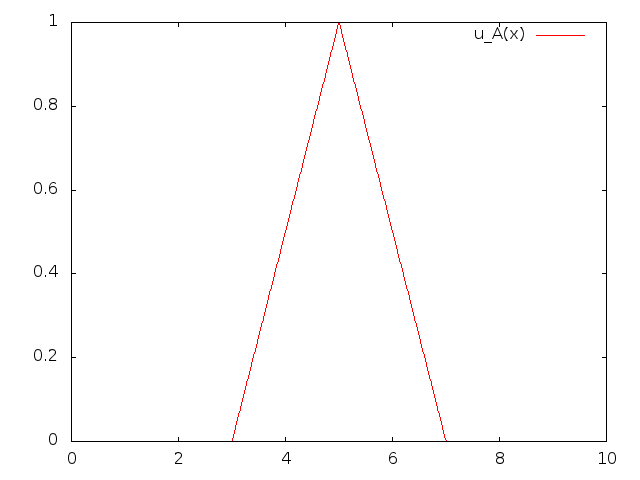
\includegraphics[scale=0.3]{ex1a.png}
        \caption{Função de pertinência.}
        \label{fig:1a}
        \end{figure}
    
    De acordo com o gráfico da função de pertinência (Figura \ref{fig:1a}), temos que seu tipo é triangular.
        

    \item[b)] Sabendo-se que a função acima está representando o conjunto referente à temperatura ``média'' de um determinado
    processo industrial, explique então qual o significado que está embutido em tal representação.

    De acordo com a representação, a temperatura média está em torno de 5 (unidade não especificada), mas com certeza não
    é menor que 3 ou maior que 7. 

    \item[c)] Explique se o conjunto \emph{fuzzy} acima é considerado um conjunto normalizado.

    O conjunto é normalizado porque pelo menos um de seus elementos possui grau de pertinência igual a 1 (elemento 5).


    \item[d)] Obtenha o conjunto suporte associado ao conjunto \emph{fuzzy} acima.

    $SUPP(A) = \{ x \in  \mathbb{R} \vert \mu_A(x) > 0\} = \{ x \in \mathbb{R} \vert x \in ]3;7[ \}$

\end{enumerate}

\item[2] Calcule a cardinalidade dos conjuntos \emph{fuzzy} discretos dados a seguir:
\begin{enumerate}
    \item[a)] $A = 0,3/x_1 + 0,5/x_2 + 0,9/x_3 + 0,4/x_4 + 0,1/x_5$

    $CARD(A) = 0,3+0,5+0,9+0,4+0,1 = 2,2 $

    \item[b)] $A = 0,0/x_1 + 0,4/x_2 + 1,0/x_3 + 1,0/x_4 + 0,4/x_5 + 0,0/x_6$

    $CARD(A) = 0,4 1,0+ 1,0 + 0,4 = 2,8$


    \item[c)] $\mu_c(x)=\frac{x}{x+1}, \text{com } x \in \{0,1,2,...,10 \}$

    $ CARD(A) = \sum\limits_{x=0}^{10}\mu_C(x) = 7,98$ 

\end{enumerate}


\item[3] Uma equipe de engenheiros e cientistas obteve a partir de experimentação diversos valores de
$\alpha$-cortes referentes a um conjunto \emph{fuzzy} V que está sendo mapeado, o qual está representando o
ajuste de vazão v de uma coluna de destilação de petróleo. Os valores referentes aos $\alpha$-cortes são
dados a seguir:\\
$V_{0.00} = {v \in \Re / 2,0 \leq v \leq 8,0}$\\
$V_{0.25} = {v \in \Re / 2,5 \leq v \leq 7,5}$\\
$V_{0.50} = {v \in \Re / 3,0 \leq v \leq 7,0}$\\
$V_{0.75} = {v \in \Re / 3,5 \leq v \leq 6,5}$\\
$V_{1.00} = {v \in \Re / 4,0 \leq v \leq 6,0}$\\
A partir das informações acima reconstrua um gráfico representativo deste conjunto, obtendo
ainda a sua expressão analítica.


\item[4] Um determinado conjunto \emph{fuzzy} deverá ser mapeado utilizando função de pertinência
triangular ou trapezoidal. Discorra sobre que subsídios você usaria para escolher uma dessas
funções para representar este conjunto. Explicite os seus argumentos através de um exemplo.


\item[5] Explique se a afirmação seguinte é verdadeira ou falsa: “Se um conjunto \emph{fuzzy} contínuo em
seu universo de discurso tiver algum de seus $\alpha$-cortes também contínuo, então o referido
conjunto é considerado convexo”.

\end{enumerate}


\end{document}
